\section{Introduction and Planning}
\subsection{Tiberius II}

This group's involvement in the Tiberius project began with Tiberius II - a four-wheeled fixed-axis variant of the robot. Comprised of an aluminium extrusion frame, four wheels and motors, a large battery pack and a number of sensors and other smaller components, this was a simplistic design from a mechanical standpoint.

\begin{figure}[!htb]
\begin{center}
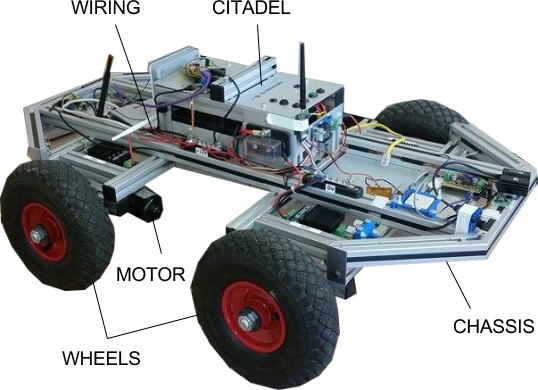
\includegraphics[width=10cm]{mech_Tib_old_diagram.png}
\end{center}
\caption{Tiberius II}
\label{fig:mech_old}
\end{figure}

However, the group unanimously decided that there was room for improvement. The aluminium frame, while simple at first glance, was in fact over-designed; using far more material than required, making the robot unnecessarily heavy and components difficult to remove or replace.

In a similar fashion the wheel and motor system left much to be desired. While simple to use, the `tank style' steering caused excessive vibrations as the robot skidded around, and the jury-rigged motors (which were salvaged windscreen wiper motors from a car) flexed under the weight of the robot.
% * <em232@hw.ac.uk> 2016-05-07T12:11:33.722Z:
%
% You would be better to say something like:  The direct drive link between the motor and the wheel meant that the coupling between the motor output shaft and the wheel shaft took the full weight of tiberius. Over time this caused the threads on the wheel shaft to be destroyed, eventually leading the the complete disconnection of the motor from the wheel.
%
% ^.

Clearly with so many changes it was likely that the entire structure of the robot would have to be changed. However, this opened up the opportunity to think about further mechanical features that would have been harder to implement while keeping the old robot intact. Drastic changes such as the addition of a steering system or shock absorbers to the frame would now be possible.

With so many opportunities for change in the pipeline it was decided that this project would culminate in an entirely new version of the Tiberius robot - dubbed `Tiberius III'.
\subsection{Aims and objectives}

With practically endless options for changing the design, it was important to plan our objectives carefully, keeping in mind the time constraints of the project. Three main areas for improvement were identified:

\begin{enumerate}
	\item Motors
	\begin{itemize}
    	\item New motors
    
    	As stated above, there were some issues with the motors on Tiberius II. As such, new motors were provided at the commencement of the project with the expectation that we would integrate them into the new design. These new DC motors are much more versatile than the old ones, and being new and of a high standard have superior power efficiency. This should improve Tiberius' power usage and increase its range.
        \newline
        The new motors include a 100:1 \gls{epicyclic gearbox}, maintaining extremely high torque while allowing them to be fixed parallel to the wheels, using very little space and removing the need for a 90\degree{} gearbox, as can be found on Tiberius II.
        \newline
        As a result, when integrated onto Tiberius the new motors provide a noticeably faster running speed - a maximum of 65 \gls{RPM}, rather than the 42 \gls{RPM} of the older motors.

    	\item Velocity control
        
        The previous version of Tiberius relied on each motor running at identical velocities to maintain a straight path. This was far from ideal, and the robot had a tendency to veer off-track, especially on rough terrain. To amend the issue, some sort of velocity control system would need to be implemented, using feedback to ensure that the motors matched each other's speed.
        
       	\item mbed control units
        
        
   	\end{itemize}
    
   	\item Wheel mounting
   	\begin{itemize}
     	\item Wheel unit
        \item Steering
        \item Suspension
   	\end{itemize}
    
	\item Chassis
   	\begin{itemize}
     	\item Reduced waste space
     	\item Refined mounts for sensors, batteries, and other equipment
     	\item Improved wiring standards
     	\item Finalised design iteration
   \end{itemize}
\end{enumerate}